\documentclass[conference]{IEEEtran}

\usepackage[utf8]{inputenc}
\usepackage[spanish, mexico, es-noindentfirst]{babel}
\usepackage[hyphens]{url}
\usepackage[caption=false,font=footnotesize]{subfig}
\usepackage{tikz}
\usetikzlibrary{arrows,
  decorations.pathmorphing,
  backgrounds,
  positioning,
  calc,
  scopes}

\addto\captionsspanish{
  \renewcommand*\IEEEkeywordsname{Palabras clave}}

\usepackage{cite}
\usepackage{amsmath,amssymb,amsfonts}
\usepackage{graphicx}
\usepackage{textcomp}
\usepackage{xcolor}
\def\BibTeX{{\rm B\kern-.05em{\sc i\kern-.025em b}\kern-.08em
    T\kern-.1667em\lower.7ex\hbox{E}\kern-.125emX}}

\begin{document}

  \title{Un vistazo a la tokenización}

  \author{%
    \IEEEauthorblockN{%
      Daniel Ayala Zamorano,
      Laura Natalia Borbolla Palacios,
      Ricardo Quezada Figueroa,
      Sandra Díaz-Santiago}
    \IEEEauthorblockA{%
      Instituto Politécnico Nacional,
      ESCOM\\
      Ciudad de México, México\\
      \textbf{\texttt{\{%
        daz23ayala,
        ln.borbolla.42,
        qf7.ricardo,
        sdiazs%
      \}@gmail.com}}}}

  \maketitle

  \begin{abstract}
    La tokenización consiste en el reemplazo de información sensible por valores
    sustitutos, llamados tokens, donde el proceso inverso, ir del  token a la
    información sensible, no es factible. En los últimos años, este proceso se
    ha vuelto muy popular entre los comercios en línea, dado que les permite
    delegar una parte de las responsabilidades de seguridad adquiridas al
    manejar números de tarjetas de crédito en un tercero: el proveedor de
    servicios de tokenización.
    Lamentablemente, existe una gran cantidad de desinformación alrededor de
    cómo generar los tokens, producida principalmente por las estrategias
    publicitarias de las empresas tokenizadoras, en donde cada una intenta
    convencer al comprador que su sistema es el mejor sin explicar realmente
    qué es lo que hacen para generar tokens. Uno de los mensajes más comunes
    entre la publicidad es que la criptografía y la tokenización son cosas
    distintas, y que la segunda es mucho más segura. En este trabajo se
    explica a detalle en qué consiste la tokenización y cuál es su relación con
    la criptografía, además, se revisa y compara el desempeño de los métodos más
    comunes para tokenizar.
  \end{abstract}

  \begin{IEEEkeywords}
    tokenización, criptografía simétrica, seguridad web
  \end{IEEEkeywords}

  \section{Introducción}

  Cuando el comercio a través de Internet comenzó a popularizarse, los fraudes
  de tarjetas bancarias se convirtieron en un problema alarmante:
  según~\cite{wallethub}, en 2001 se tuvieron pérdidas de de 1.7 mil millones de
  dólares y para 2002 aumentaron a 2.1 mil millones. En este contexto, el {\it
  Payment Card Industry Security Standard Council (PCI SSC)}, integrado por las
  principales compañías de tarjetas de crédito, desarrolla el estándar
  \textit{Payment Card Industry Data Security Standard (PCI
  DSS)}~\cite{pci_dss}), con el propósito de especificar mecanismos de seguridad
  para proteger los datos sensibles de las tarjetas de crédito. Sin embargo,
  satisfacer los requerimientos establecidos en dicho estándar es sumamente
  difícil, especialmente para los negocios pequeños y medianos. Esto se debe a
  que la información sensible debe protegerse en donde sea que se encuentre, al
  almacenarla, transmitirla y/o procesarla. A pesar de la publicación del
  estándar en 2004, las grandes filtraciones de datos no han cesado:
  \textit{TJX} en 2006, \textit{Hannaford Bros.} en 2008, \textit{Target} en
  2013 y \textit{Home Depot} en 2014, por mencionar algunos
  ejemplos~\cite{wallethub}.

  Ante este escenario surge un nuevo paradigma, denominado {\it tokenización},
  el cual consiste en reemplazar los datos sensibles por un {\it token}, es
  decir, un valor numérico o alfabético que no tiene relación alguna con el dato
  original. En este paradigma, la información sensible se concentra  en un solo
  lugar para hacer la tarea de protección más sencilla; así, cuando se ingresa
  un nuevo valor sensible, e.g. un número de tarjeta de un usuario, se genera un
  token ligado a esa información; el token se usa en todo el sistema y la
  información sensible se protege en un solo lugar. Un posible adversario con
  acceso a los tokens no podrá obtener la información sensible a partir de
  estos.

  Una de las ventajas de la tokenización es que puede verse como un sistema
  autónomo, independiente al sistema principal; de esta manera se establece una
  separación de responsabilidades: el sistema principal realiza la operación del
  negocio (por ejemplo, una tienda en línea) y el sistema tokenizador se dedica
  a la protección de la información sensible. Hoy en día, varias compañías
  ofrecen servicios de tokenización que permiten que los comerciantes se liberen
  casi por completo de cumplir con el PCI DSS. En la
  Figura~\ref{figura:arquitectura_tokenizacion}, se muestra una distribución
  bastante común para un comercio en línea: el sistema tokenizador guarda la
  información sensible en su base de datos y se encarga de realizar las
  transacciones bancarias.

  Aunque esta solución parece apropiada, aún es necesario responder preguntas
  tales como ¿cuáles son los mecanismos para generar tokens?, ¿cuál es su nivel
  de desempeño?, ¿cuáles son las implicaciones de seguridad al utilizar algún
  algoritmo en particular? Desafortunadamente, la tokenización se ha visto
  rodeada por una nube de desinformación desde sus inicios; la falta de una
  definición formal permitió que las campañas publicitarias de las empresas
  tokenizadoras difundieran información imprecisa: se suele mencionar que la
  tokenización y la criptografía no están relacionadas directamente, o bien, que
  la primera es una alternativa (y no una aplicación) de la segunda. Por
  ejemplo, lo único que \textit{Shift4} dice con claridad sobre sus tokens, es
  que se trata de valores aleatorios, únicos y alfanuméricos \cite{shif4_uno};
  para \textit{Braintree}, la única manera de generar tokens es por métodos
  aleatorios \cite{braintree_uno}; finalmente, para \textit{Securosis} los
  tokens son valores aleatorios que nada tienen que ver con la criptografía
  \cite{securosis}; es fácil observar que la mayoría de las empresas trata a sus
  métodos como secretos de compañía, esperando que el trato entre cliente y
  proveedor esté basado en la confianza y no en la comparación de los propios
  métodos tokenizadores.

  Afortunadamente, ya se han dado los primeros pasos para responder a las
  preguntas antes planteadas. Hasta el momento se han propuesto diversas
  soluciones para generar tokens, las cuales están basadas en primitivas
  criptográficas y también se ha comenzado a analizar la seguridad de tales
  soluciones. El presente artículo ofrece una breve descripción de los
  principales algoritmos para generar tokens, los cuales están basados, en
  funciones hash, cifrados por bloque y cifrados que preservan el formato, entre
  otros. También se analiza la eficiencia de los mismos, con la finalidad de
  ofrecer un punto de comparación entre ellos.

  En la Sección~\ref{sec:preliminares} se definen las primitivas criptográficas
  que utilizan los distintos algoritmos para generar tokens; en la
  Sección~\ref{sec:algoritmos}, se da una breve descripción de los métodos de
  tokenización implementados. Finalmente, en la Sección~\ref{sec:conclusiones},
  se presentan los resultados de las comparaciones de desempeño realizadas y se
  concluye con una discusión alrededor del tema.

  \begin{figure}
    \centering
    \begin{tikzpicture}[
      entorno/.style={
        rectangle,
        draw = black,
        thin,
        inner sep = 1mm,
        text width = 20mm,
        align = center,
        minimum height = 1.2cm},
      etiqueta/.style={
        text width = 15mm,
        align = center
      }]

      % Entornos
      \node[entorno]
        (tokens)
        {\footnotesize Sistema tokenizador};
      \node[entorno]
        (tienda)
        [right = 2.5cm of tokens]
        {\footnotesize Entorno de comerciante};
      \node[entorno]
        (banco)
        [below = 1.2cm of tokens]
        {\footnotesize Entorno de banco};
      \node[entorno]
        (usuario)
        [below = 1.2cm of tienda]
        {\footnotesize Cliente};

      % Comunicación
      \draw[-stealth',
        transform canvas = {
          yshift=6pt}]
        (tienda.west)
        --
        node[
          etiqueta,
          above]
          {\footnotesize Número de tarjeta}
        (tokens.east);
      \draw[-stealth',
        transform canvas = {
          yshift=-6pt}]
        (tokens.east)
        --
        node[
          etiqueta,
          below]
          {\footnotesize Token}
        (tienda.west);
      \draw[-stealth']
        (tokens.south)
        --
        node[
          etiqueta,
          left]
          {\footnotesize Número de tarjeta}
        (banco.north);
      \draw[-stealth']
        (usuario.north)
        --
        node[
          etiqueta,
          right]
          {\footnotesize Número de tarjeta}
        (tienda.south);

    \end{tikzpicture}
    \caption{Arquitectura típica de un sistema tokenizador.}
    \label{figura:arquitectura_tokenizacion}
  \end{figure}

  \section{Preliminares}
  \label{sec:preliminares}

  \subsection{Notación}

  Se denotará  a todas las cadenas de bits de longitud $ n $ como $ \{ 0, 1 \}^n
  $ y a las cadenas de longitud arbitraria como $ \{ 0, 1 \}^* $. Para una
  cadena de símbolos $ x $ sobre un alfabeto arbitrario, $ | x | $ simboliza la
  longitud de la cadena. La expresión $ f: \mathcal{X} \rightarrow \mathcal{Y} $
  denota a una función $ f $ que asigna a cada elemento del conjunto $
  \mathcal{X} $ un elemento del conjunto $ \mathcal{Y} $. La expresión $
  \mathcal{A} \times \mathcal{B} $, en donde $ \mathcal{A} $ y $ \mathcal{B} $
  son conjuntos, denota al producto cartesiano, esto es, $ \mathcal{A} \times
  \mathcal{B} = \{ (a,b) \ | \ a \in \mathcal{A} \land b \in \mathcal{B} \} $.

  \subsection{Primitivas criptográficas}

  Un cifrador por bloques se define como una función $ e: \mathcal{M} \times
  \mathcal{K} \rightarrow \mathcal{C} $ donde $ \mathcal{M} = \mathcal{C} = \{
    0, 1 \}^n $, $ \mathcal{K} = \{ 0, 1 \}^k $, $ n $, es el tamaño del bloque
  y $ k $, el tamaño de la llave~\cite{menezes}.

  Los modos de operación permiten extender la funcionalidad de los cifrados por
  bloque para poder operar sobre bloques de información de tamaño arbitrario.
  Más formalmente, un modo de operación~\cite{modos_de_operacion} es un
  procedimiento que recibe como entrada un mensaje de longitud arbitraria $ M
  \in \{ 0, 1 \}^*$, una llave $ K \in \{0, 1 \}^k$, un vector de inicialización
  $IV \in \{ 0, 1 \}^v $ y da como salida un texto cifrado $C \in \{ 0, 1 \}^*
  $.

  Una función \textit{hash} criptográfica asocia cadenas de longitud arbitraria
  a cadenas de longitud fija: $ H:  \{ 0, 1 \}^* \rightarrow \{ 0, 1 \}^h $,
  donde $h$ es la longitud de la cadena de salida, también denominada resumen o
  digesto.  No debe ser factible recuperar el mensaje a partir de su valor
  \textit{hash}, ni encontrar dos mensajes que produzcan el mismo
  \textit{hash}~\cite{menezes}.

  Un código de autenticación de mensaje (MAC, \textit{Message Authentication
  Code}) es una primitiva criptográfica que provee integridad. Se define como
  una tupla de tres algoritmos: generación de claves, generación de la etiqueta
  y verificación de la etiqueta. El algoritmo para generar la etiqueta, recibe
  como entrada una llave $K \in \mathcal{K}$ y un mensaje $M \in \{ 0, 1 \}^*$ y
  como salida se obtiene una etiqueta $\tau \in \{ 0, 1 \}^t$. El algoritmo de
  verificación recalcula una etiqueta $\tau^\prime$, a partir del mensaje $M$ y
  la llave $K$, y la compara con la etiqueta $\tau$: si ambas son iguales, se
  dice que el mensaje no ha sido modificado.

  Las redes Feistel son cifrados iterativos que transforman un texto en claro de
  $ 2t $ bits denominado $ (L_0, R_0) $, en donde $ L_0 $ y $ R_0 $ son bloques
  de $ t $ bits, en un texto cifrado $ (R_r, L_r) $ a través de un proceso de $
  r $ rondas. Existen dos generalizaciones de este concepto, las redes
  alternantes y las redes desbalanceadas; ambas permiten modificar el tamaño de
  las mitades izquierda y derecha: $ 1 \geq | L_n | \leq 2t $ y $ | R_n | = 2t -
  | L_n | $~\cite{DBLP:conf/fse/SchneierK96}.

  Un cifrado que preserva el formato (en inglés \textit{Format-preserving
  Encryption}, FPE) es un cifrado simétrico en donde el mensaje en claro y el
  mensaje cifrado mantienen un formato en común. Formalmente, de acuerdo a lo
  definido en~\cite{DBLP:conf/sacrypt/BellareRRS09}, se trata de una función $
  E: \mathcal{K} \times \mathcal{N} \times \mathcal{T} \times \mathcal{X}
  \rightarrow \mathcal{X} $, en donde los conjuntos $ \mathcal{K} $, $
  \mathcal{N} $, $ \mathcal{T} $, $ \mathcal{X} $ corresponden al espacio de
  llaves, espacio de formatos, espacio de \textit{tweaks} y el dominio,
  respectivamente. El proceso de cifrado de un elemento del dominio con respecto
  a una llave $ K $, un formato $ N $ y un \textit{tweak} $ T $ se escribe como
  $ E_K^{N,T}(X) $. El proceso inverso es también una función $ D: \mathcal{K}
  \times \mathcal{N} \times \mathcal{T} \times \mathcal{X} \rightarrow
  \mathcal{X} $, en donde $ D_K^{N,T}\big( E_K^{N,T}(X) \big) = X $.

  \section{Algoritmos tokenizadores}
  \label{sec:algoritmos}

  En el presente artículo se trata a la generación de tokens como un servicio,
  ver Figura~\ref{figura:arquitectura_tokenizacion}, por lo que la interfaz para
  los procesos de tokenización y detokenización, desde el punto de vista del
  usuario, se define como sigue:  el proceso para generar un token es una
  función $ E: \mathcal{X} \rightarrow \mathcal{Y} $ y el proceso para recuperar
  al número de tarjeta es simplemente la función inversa $ D: \mathcal{Y}
  \rightarrow \mathcal{X} $, en donde $ \mathcal{X} $ y $ \mathcal{Y}$ son los
  espacios de números de tarjetas y tokens, respectivamente. Los números de
  tarjetas bancarias cuentan con entre 12 y 19 dígitos, y están normados por el
  estándar ISO/IEC-7812~\cite{iso_7812}.

  \subsection{Clasificación del PCI SSC} \label{sec:clasificacion}

  El PCI SSC establece en sus guías de tokenización la siguiente clasificación
  para los algoritmos tokenizadores~\cite{pci_tokens}:

  \begin{itemize}
    \item Métodos reversibles. Aquellos para los cuales es posible obtener el
      número de tarjeta a partir del token.
      \begin{itemize}
        \item Criptográficos. El proceso de tokenización está basado en un
          esquema de cifrado simétrico que usa el número de tarjeta y una llave
          para obtener un token. El proceso de detokenización solicitará el
          token y la misma llave para recuperar el número de tarjeta.
        \item No criptográficos. Se requiere una base de datos para guardar las
          relaciones entre números de tarjetas y tokens; el proceso de
          detokenización es una consulta a la base de datos.
      \end{itemize}
    \item Métodos irreversibles. Aquellos en los que no es posible obtener el
      número de tarjeta original a partir del token.
      \begin{itemize}
        \item Autenticable. Permiten validar cuando un token dado corresponde a
          un número de tarjeta.
        \item No autenticable. No permiten hacer la validación anterior.
      \end{itemize}
  \end{itemize}

  \subsection{Algoritmos implementados}
  \label{sec:implementaciones}

  En esta sección se describen brevemente algunas de las soluciones que han sido
  propuestas por la comunidad académica para generar tokens. La primera de ellas
  está basada en cifrados que preservan el formato, en particular en FFX y BPS,
  los cuales ya forman parte de los estándares del NIST (\textit{National
  Institute of Standards and Technology})~\cite{nist_fpe}. La ventaja de este
  mecanismo es que no se requiere de una base de datos para recuperar el número
  de tarjeta de crédito, basta con descifrar el token.

  FFX (\textit{Format-preserving Feistel-based Encryption}) fue presentado
  en~\cite{ffx_1} por Bellare, Rogaway y Spies. Este algoritmo permite cifrar
  cadenas de cualquier longitud en cualquier alfabeto; en particular, se
  consideran alfabetos binarios y alfabetos decimales, denominados A2 y A10,
  respectivamente. FFX A10 usa una red Feistel alternante junto con una
  adaptación de AES-CBC-MAC (usada como función de ronda) para lograr preservar
  el formato. Brier, Peyrin y Stern propusieron el algoritmo BPS~\cite{bps}. Se
  conforma de 2 partes: un cifrado interno $BC$ que cifra bloques de longitud
  fija y un modo de operación especial, encargado de extender la funcionalidad
  de $BC$ y de permitir cifrar cadenas de mayor longitud.

  En 2016, Díaz et. al.~\cite{doc_sandra} analizaron el problema de la
  generación de tokens desde el punto de vista criptográfico y propusieron un
  algoritmo (TKR) que no está basado en cifrados que preservan el formato. Hasta
  antes de la publicación de este documento, los únicos métodos para generar
  tokens cuya seguridad estaba formalmente demostrada eran los basados en
  cifrados que preservan el formato.  El algoritmo propuesto usa un cifrado por
  bloques para generar tokens pseudoaleatorios y almacena en una base de datos
  la relación original de estos con los números de tarjetas. El proceso de
  detokenización es simplemente una consulta sobre la base de datos.

  En 2017, Longo, Aragona y Sala~\cite{aragona} propusieron un algoritmo que
  denominaron \textit{híbrido reversible} (AHR) que está basado en un cifrador
  por bloques y utiliza una base de datos para almacenar las relaciones entre
  número de tarjeta y token. Las entradas del algoritmo son la parte del número
  de tarjeta a cifrar y una entrada adicional (por ejemplo, la fecha) que
  permite que se tengan varios tokens relacionados con la misma tarjeta. Como se
  desea obtener un token que tenga el mismo número de dígitos que la tarjeta
  ingresada, se utiliza un método llamado \textit{caminata cíclica}
  \cite{blackrog} para asegurarse de que el texto cifrado pertenezca al espacio
  del texto en claro.

  Probablemente el método más directo para generar tokens es mediante un DRBG
  (\textit{Deterministic Random Bit Generator}). La idea es producir una cadena
  binaria aleatoria con un DRBG e interpretarla para que tenga el formato de un
  token. Para este trabajo se hizo la implementación de dos DRBG: uno basado en
  SHA y otro basado en un cifrado por bloques; ambos definidos en el estándar
  del NIST 800-90A~\cite{nist_aleatorios}.

  El método que utiliza como mecanismo interno a una función \textit{hash}
  consiste en ir concatenando de forma consecutiva los valores \textit{hash}
  derivados de la semilla e ir incrementando el valor de esta. El método basado
  en un cifrado por bloques utiliza el modo de operación CTR, en donde la
  semilla juega el papel de vector de inicialización. En ambos casos, la
  seguridad se basa en que la semilla sea un valor secreto.

  Según la clasificación del PCI DSS, FFX y BPS son %(Sección
  \ref{sec:clasificacion}) algoritmos reversibles criptográficos, ya que al ser
  cifrados que preservan el formato, funcionan como esquema de cifrado
  simétrico. TKR, AHR y DRBG son, contradictoriamente, reversibles no
  criptográficos, pues necesitan de una base de datos para guardar las
  relaciones tarjeta-token.

  \section{Resultados y conclusiones}
  \label{sec:conclusiones}

  \begin{table}
    \renewcommand{\arraystretch}{1.3}
    \centering
    \caption{Comparación de tiempos de tokenización.}
    \label{tabla:tiempos_tokenizacion}
    \begin{tabular}{c c c}
      \hline
       & Tokenización ($\mu$s) & Detokenización ($\mu$s) \\
      \hline
      FFX & 83 & 61 \\
      BPS & 573 & 315 \\
      TKR & 4648 & 281 \\
      AHR & 5554 & 657 \\
      DRBG & 4649 & 431 \\
      \hline
    \end{tabular}
  \end{table}

  En la Tabla \ref{tabla:tiempos_tokenizacion} y la Figura
  \ref{figura:tiempos_unitarios} se muestran los resultados en tiempo de las
  ejecuciones de los algoritmos presentados en la Sección
  \ref{sec:implementaciones}. Estos se llevaron a cabo en una computadora con
  las siguientes características:

  \begin{itemize}
    \item \textbf{Procesador:} Intel i5-7200U (2.5 GHz) de 4 núcleos.
    \item \textbf{Sistema operativo:} Arch Linux, kernel 4.17.
    \item \textbf{Base de datos:} MariaDB 10.1.
    \item \textbf{Compilador:} GCC 8.1.1.
  \end{itemize}

  El procesador utilizado soporta los conjuntos de instrucciones de Intel AES-NI
  y RD-SEED~\cite{aesni_wp}. Los algoritmos tokenizadores que usan un cifrado
  por bloques utilizan una implementación de AES con las instrucciones a nivel
  de hardware. El DRBG se implementó haciendo uso de la instrucción RD-RAND como
  fuente de entropía.

  La comparación de la Figura \ref{figura:tiempos_unitarios} muestra como los
  dos algoritmos reversibles, FFX y BPS, son considerablemente más rápidos que
  los tres irreversibles: TKR, AHR y DRBG. Los reversibles están en el rango de
  60 a 170 microsegundos, mientras que los irreversibles están en alrededor de
  los 5500 microsegundos. También es posible observar que, para los métodos
  irreversibles, el proceso de detokenización es mucho más rápido que la
  generación de tokens.  Estos dos resultados dejan ver un poco la carga de las
  operaciones en los métodos irreversibles: la tokenización involucra una
  consulta a la base, la generación del token y una inserción; la detokenización
  solamente es una consulta.

  El que FFX y BPS sean más rápidos puede resultar un poco contraintuitivo, pues
  la generación de tokens reversibles involucra más operaciones; es por esto que
  en la Figura \ref{figura:tiempos_tokenizacion} se muestran los tiempos de la
  generación de tokens, sin tomar en cuenta tiempos de acceso a base de datos.
  En este caso, el más veloz es DRBG, seguido de cerca por TKR y AHR; los dos
  reversibles van al último.

  Además de los tiempos de ejecución, también es importante señalar que los
  irreversibles, al operar como funciones de un solo sentido, son más seguros
  que los reversibles: un atacante con acceso a la llave de cifrado puede
  obtener el número de tarjeta correspondiente si se trata de un método
  reversible, mientras que con un método irreversible necesita también acceso a
  la base de datos.

  La denominación \textit{no criptográficos}, de la clasificación del PCI DSS
  resulta totalmente confusa, pues en realidad todos los métodos conocidos que
  caen en esa categoría utilizan primitivas criptográficas. La segunda categoría
  (irreversibles) carece de utilidad para aplicaciones que procesan pagos con
  tarjetas de crédito, pues la habilidad de regresar al número de tarjeta a
  partir de su token es uno de los requerimientos principales para los sistemas
  tokenizadores. Por lo anterior, en este trabajo se propone una clasificación
  distinta:

  \begin{itemize}
    \item Métodos criptográficos. Todos aquellos basados en primitivas
      criptográficas.
      \begin{itemize}
        \item Reversibles. Usan un esquema de cifrado simétrico. El mecanismo de
          tokenización cifra el número de tarjeta y la detokenización descifra
          el token para obtener el número de tarjeta original.
        \item Irreversibles. Hacen uso de algoritmos criptográficos para generar
	        el token y herramientas externas, como una base de datos, para guardar
          las relaciones entre tokens y números de tarjetas.
      \end{itemize}
    \item Métodos no criptográficos. Aquellos  métodos que no necesitan
      herramientas relacionadas con la criptografía; por ejemplo, un generador
      de números realmente aleatorio (TRNG, \textit{True Random Number
      Generator}).
  \end{itemize}

  \begin{figure}[!t]
    \centering
    \subfloat[Tokenización y detokenización]{
      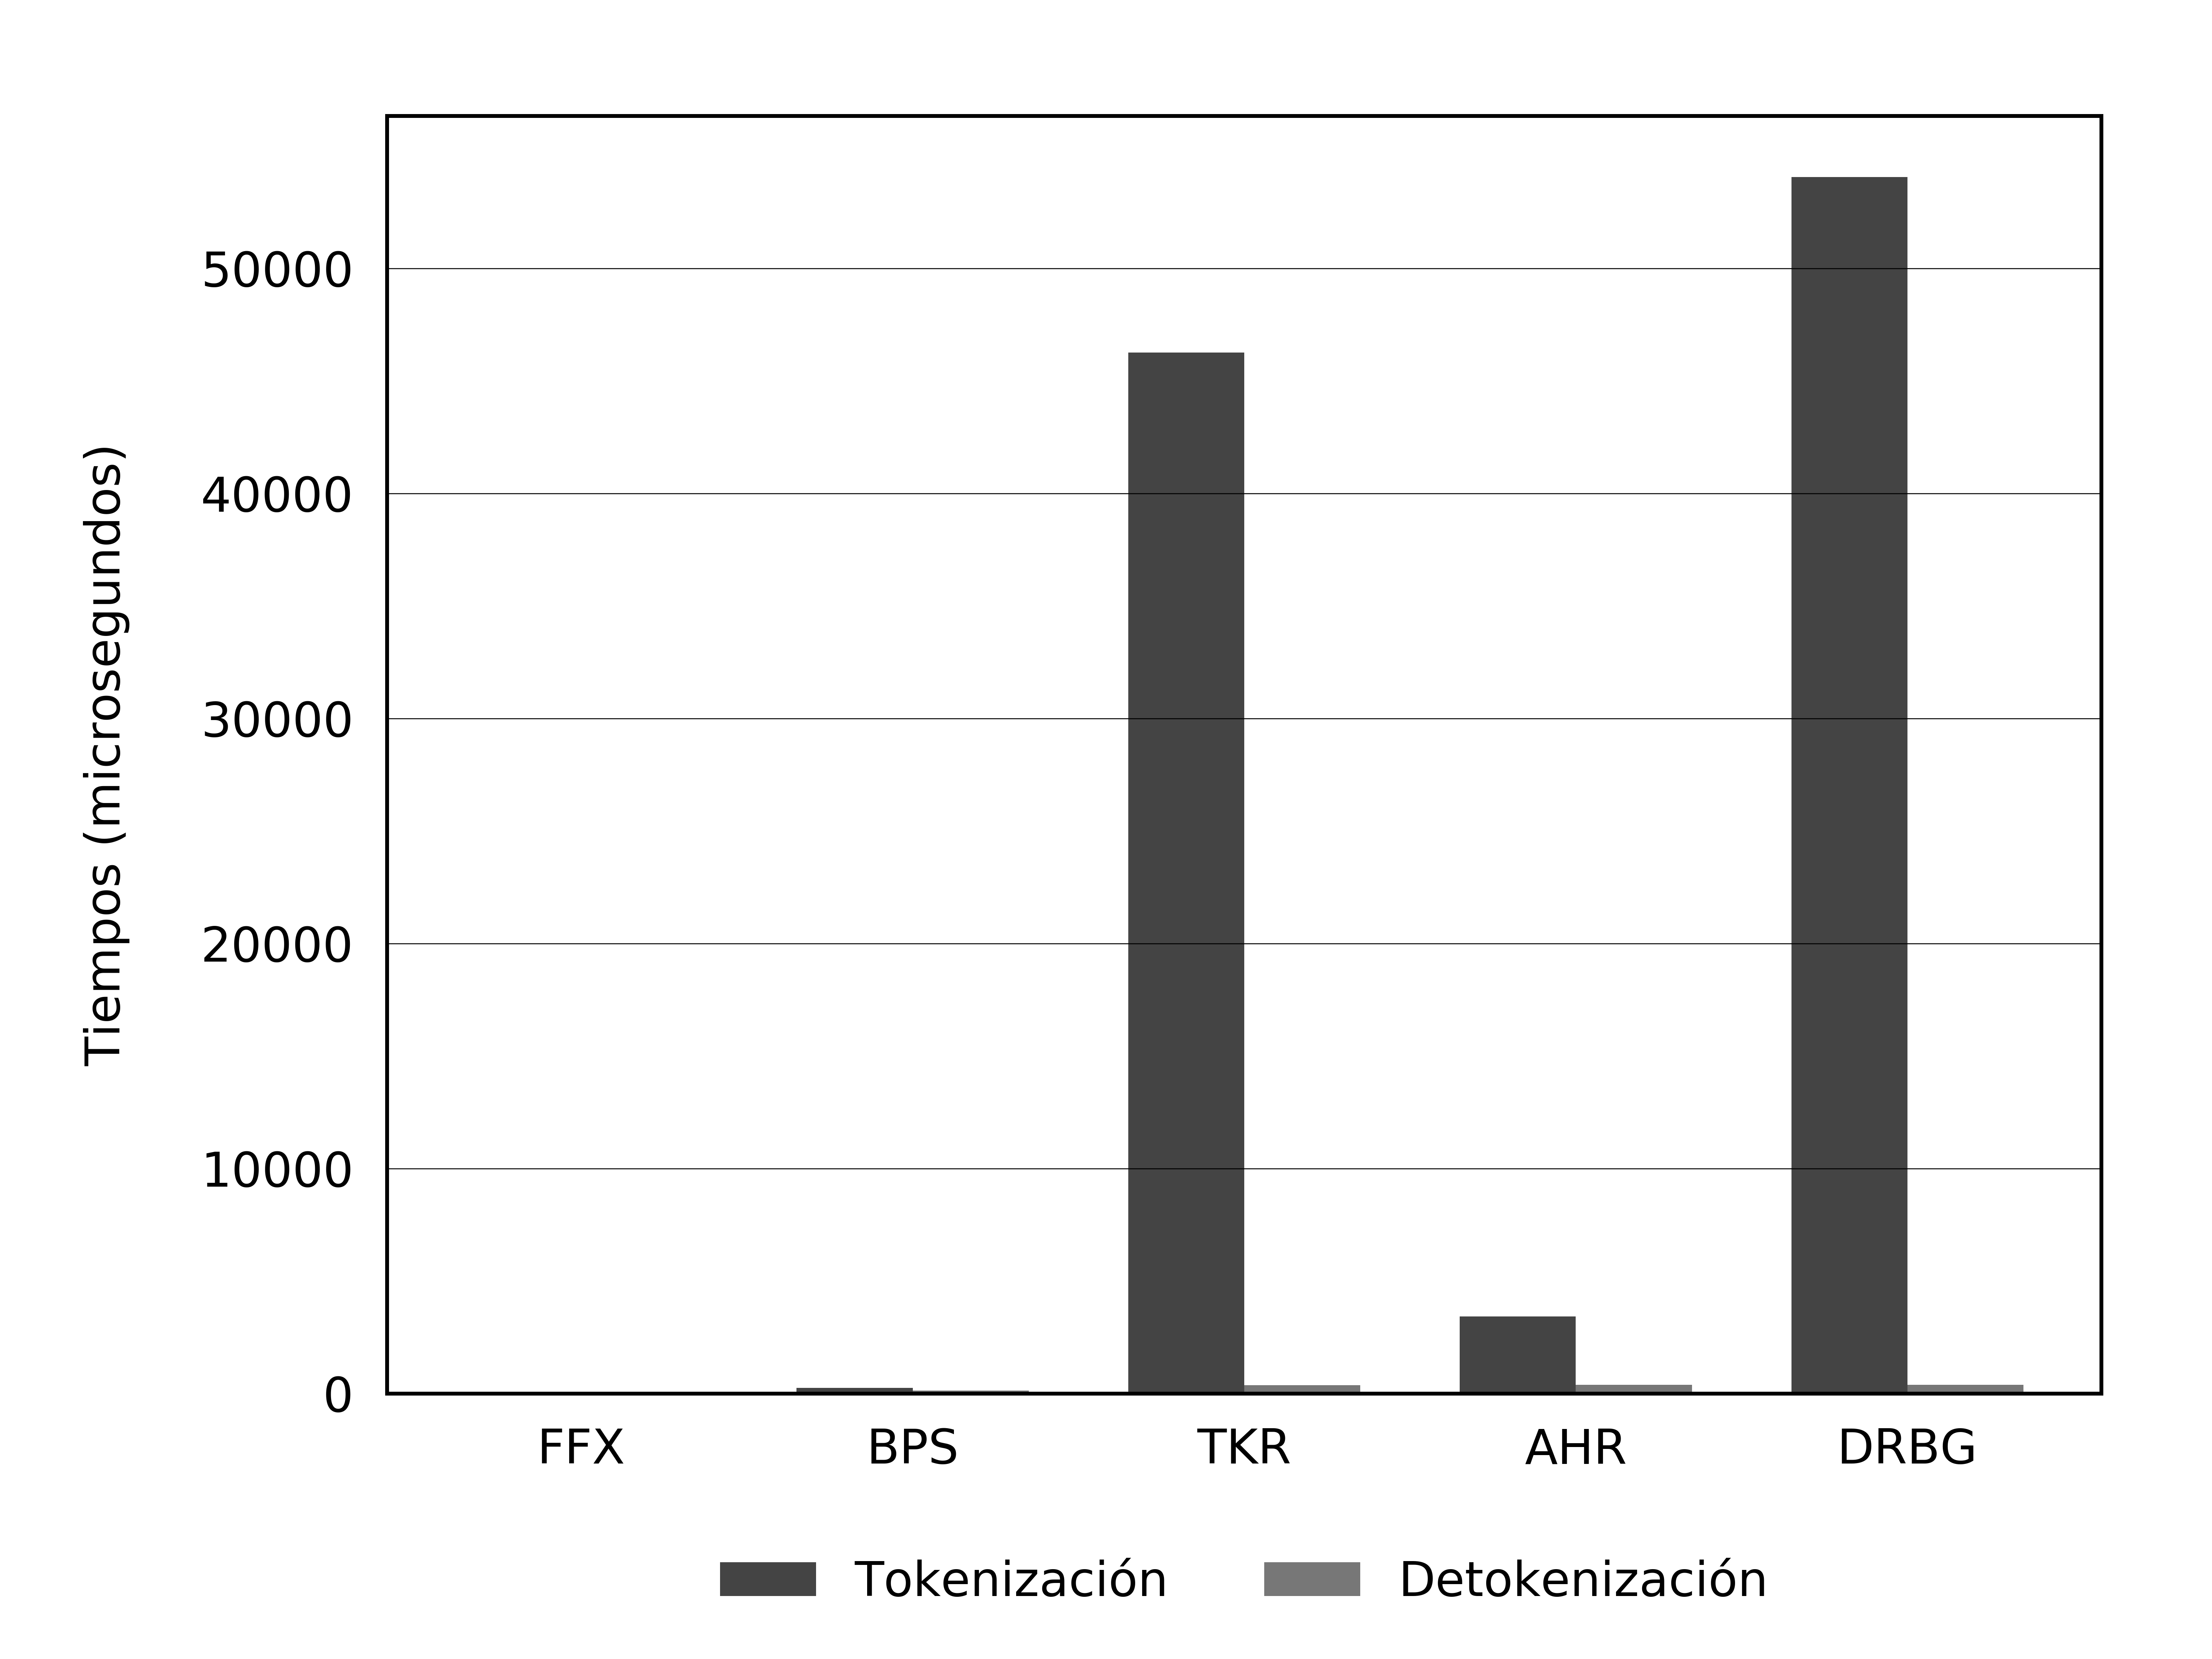
\includegraphics[width=3.1in]
        {tiempos_unitarios.png}
      \label{figura:tiempos_unitarios}}
    \\
    \subfloat[Generación de tokens]{
      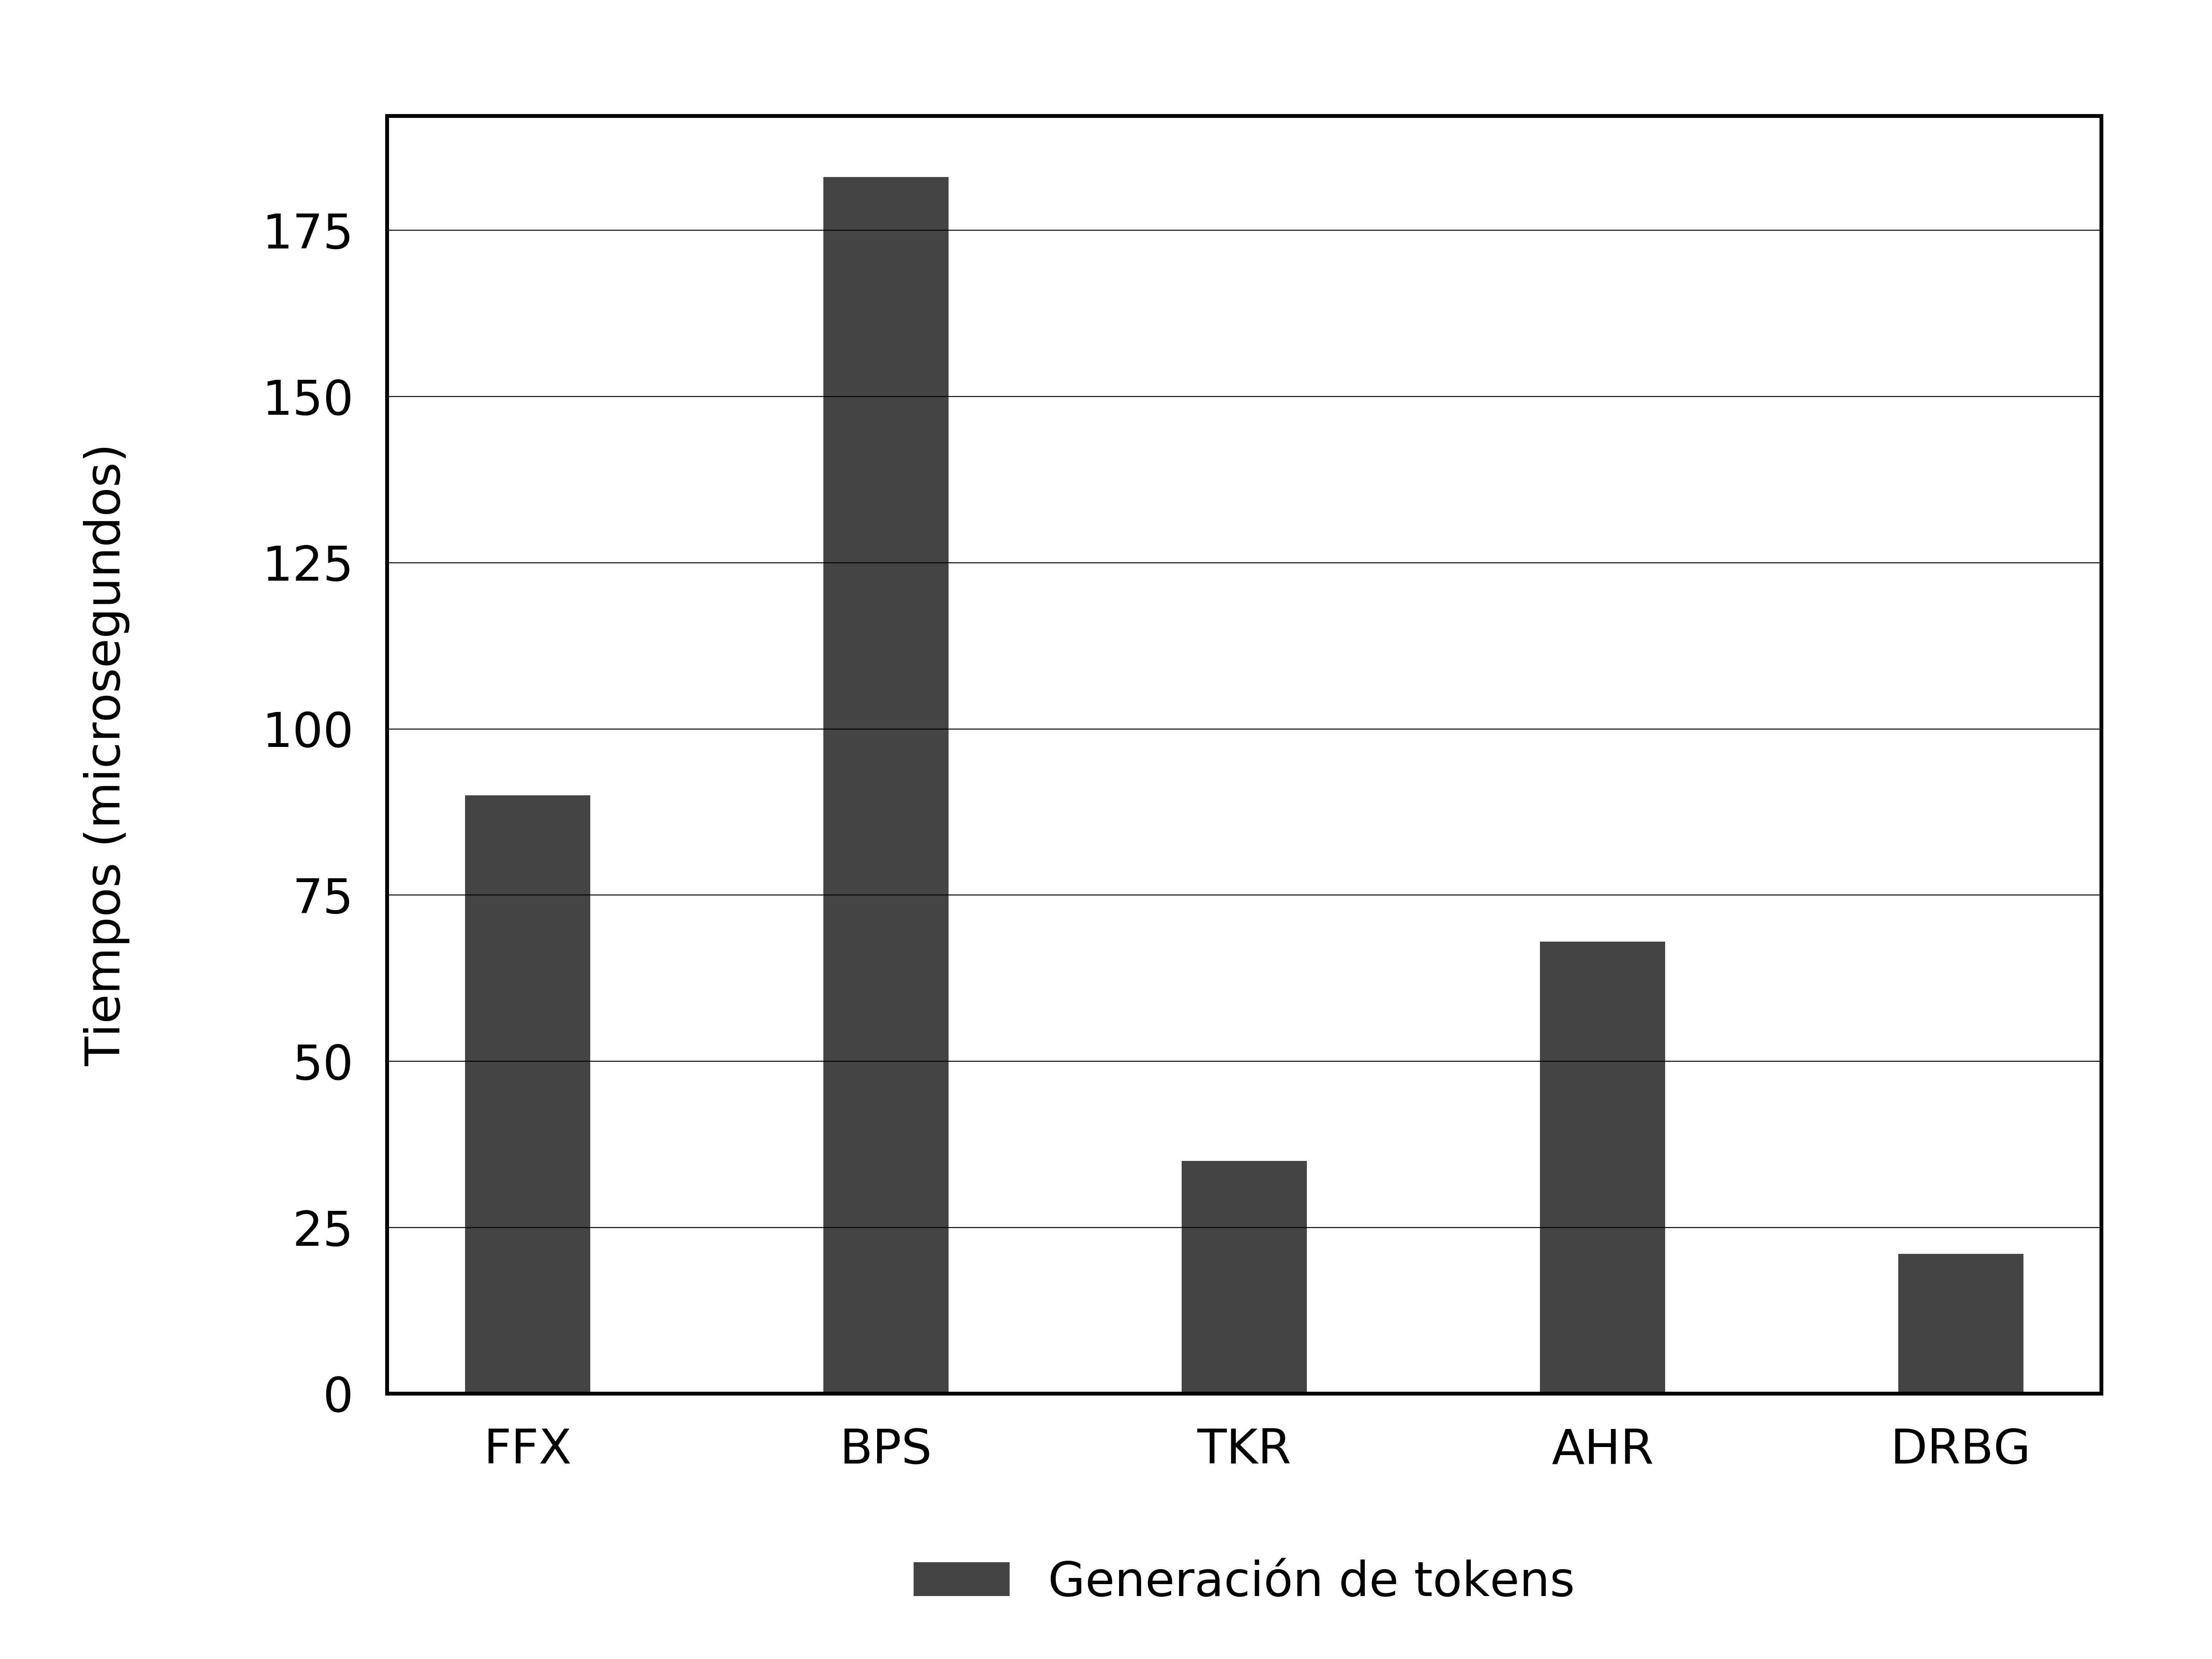
\includegraphics[width=3.1in]
        {tiempos_tokenizacion.png}
      \label{figura:tiempos_tokenizacion}}
    \caption{Comparaciones de tiempos.}
    \label{fig_sim}
  \end{figure}

  \section*{Agradecimientos}

  Los autores agradecen el apoyo del Instituto Politécnico Nacional, a través
  del proyecto multidisciplinario SIP 1917, módulo 20180775.

  \bibliographystyle{abbrv}
  \bibliography{referencias}

\end{document}

